%
% Copyright 2018 Joel Feldman, Andrew Rechnitzer and Elyse Yeager.
% This work is licensed under a Creative Commons Attribution-NonCommercial-ShareAlike 4.0 International License.
% https://creativecommons.org/licenses/by-nc-sa/4.0/
%
\questionheader{ex:s3.4.1}


%%%%%%%%%%%%%%%%%%
\subsection*{\Conceptual}
%%%%%%%%%%%%%%%%%%



\begin{Mquestion}
The graph below shows three curves. The black curve is $y=f(x)$, the red curve is $y=g(x)=1+2\sin(1+x)$, and the blue curve is $y=h(x)=0.7$. If you want to estimate $f(0)$, what might cause you to use $g(0)$? What might cause you to use $h(0)$?
\begin{center}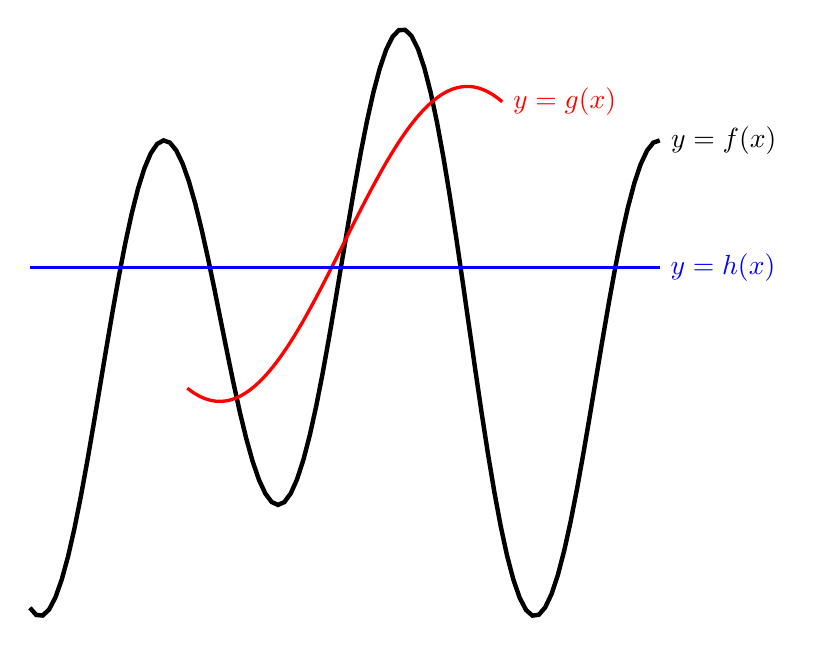
\begin{tikzpicture}
\YEaxis{4}{4}
\draw[ultra thick, black] plot[domain=-4:4, samples=100](\x,{3*sin(2*\x r)+cos(\x r)}) node[right]{$y=f(x)$};
\draw[very thick, red] plot[domain=-2:2, samples=100](\x,{1+2*sin(1+\x r)}) node[right]{$y=g(x)$};
\draw[very thick, blue] plot[domain=-4:4, samples=100](\x,{.7}) node[right]{$y=h(x)$};
\end{tikzpicture}\end{center}
\end{Mquestion}
\begin{hint}
An approximation should be something you can actually figure out--otherwise it's no use.
\end{hint}
\begin{answer}
Since $f(0)$ is  closer to $g(0)$ than it is to $h(0)$, you would probably want to estimate $f(0) \approx g(0)=1+2\sin (1)$ if you had the means to efficiently figure out what $\sin(1)$ is, and if you were concerned with accuracy. If you had a calculator, you could use this estimation. Also, later in this chapter we will learn methods of approximating $\sin (1)$ that do not require a calculator, but they do require time.

Without a calculator, or without a lot of time, using $f(0)\approx h(0)=0.7$ probably makes the most sense. It isn't as accurate as $f(0) \approx g(0)$, but you get an estimate very quickly, without worrying about figuring out what $\sin(1)$ is.
\end{answer}
\begin{solution}
Since $f(0)$ is  closer to $g(0)$ than it is to $h(0)$, you would probably want to estimate $f(0) \approx g(0)=1+2\sin (1)$ if you had the means to efficiently figure out what $\sin(1)$ is, and if you were concerned with accuracy. If you had a calculator, you could use this estimation. Also, later in this chapter we will learn methods of approximating $\sin (1)$ that do not require a calculator, but they do require time.

Without a calculator, or without a lot of time, using $f(0)\approx h(0)=0.7$ probably makes the most sense. It isn't as accurate as $f(0) \approx g(0)$, but you get an estimate very quickly, without worrying about figuring out what $\sin(1)$ is.

Remark: when you're approximating something in real life, there probably won't be an obvious ``correct" way to do it. There's usually a trade-off between accuracy and ease.
\end{solution}




%%%%%%%%%%%%%%%%%%
\subsection*{\Procedural}
%%%%%%%%%%%%%%%%%%
\Instructions{
In this and following sections, we will ask you to approximate the value of several constants, such as $\log(0.93)$. A valid question to consider is why we would ask for approximations of these constants that take lots of time, and are less accurate than what you get from a calculator. }

\Instructions{One answer to this question is historical: people were approximating logarithms before they had calculators, and these are some of the ways they did that. Pretend you're on a desert
             island without any of your usual devices and that you
             want to make a number of quick and dirty approximate
             evaluations.}

\Instructions{Another reason to make these approximations is technical: how does the \emph{calculator} get such a good approximation of $\log(0.93)$? The techniques you will learn later on in this chapter give very accurate formulas for approximating functions like $\log x$ and $\sin x$, which are sometimes used in calculators. }

\Instructions{A third reason to make simple approximations of expressions that a calculator could evaluate is to provide a reality check. If you have a ballpark guess for your answer, and your calculator gives you something wildly different, you know to double-check that you typed everything in correctly.}

\Instructions{For now, questions like
Question~\ref{s3.4.1startapprox} through
Question~\ref{s3.4.1endapprox} are simply for you to practice the fundamental ideas we're learning.}

\begin{question}\label{s3.4.1startapprox}
Use a constant approximation to estimate the value of $\log(x)$ when $x=0.93$. Sketch the curve $y=f(x)$ and your constant approximation.

(Remember that in CLP-1 we use $\log x$ to mean the natural logarithm of $x$, $\log_e x$.)
\end{question}
\begin{hint}
You'll need some constant $a$ to approximation $\log(0.93) \approx \log(a)$.
This $a$ should have two properties: it should be close to 0.93, and you should be able to easily evaluate $\log(a)$.
\end{hint}
\begin{answer}
$\log(0.93)\approx \log(1)=0$
 \begin{center}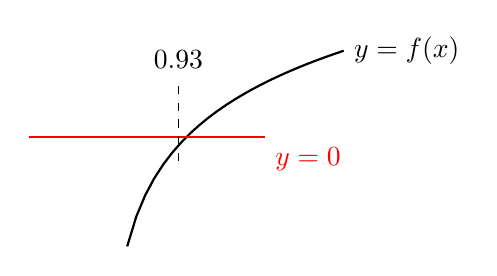
\begin{tikzpicture}
 \YEaaxis{1.5}{3.5}{1}{2}
 \draw[thick] plot[domain=0.25:3](\x,{ln \x}) node[right]{$y=f(x)$};
 \draw[thick, red] (-1,0)--(2,0) node[below right]{$y=0$};
 \draw[dashed] (.9,-.3)--(.9,.75) node[above]{0.93};
 \YExcoord{1}{1}
 \end{tikzpicture}\end{center}

\end{answer}
\begin{solution}
 0.93 is pretty close to 1, and we know $\log(1)=0$, so we estimate
 $\log(0.93) \approx \log(1)=0$.
 \begin{center}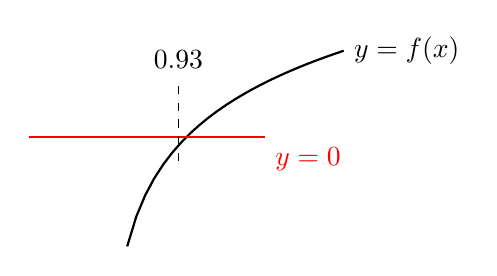
\begin{tikzpicture}
 \YEaaxis{1.5}{3.5}{1}{2}
 \draw[thick] plot[domain=0.25:3](\x,{ln \x}) node[right]{$y=f(x)$};
 \draw[thick, red] (-1,0)--(2,0) node[below right]{$y=0$};
 \draw[dashed] (.9,-.3)--(.9,.75) node[above]{0.93};
 \YExcoord{1}{1};
 \end{tikzpicture}\end{center}
\end{solution}




\begin{Mquestion}
Use a constant approximation to estimate
$\arcsin(0.1)$.
\end{Mquestion}
\begin{hint}
You'll need some constant $a$ to approximate $\arcsin(0.1) \approx \arcsin(a)$.
This $a$ should have two properties: it should be close to 0.1, and you should be able to easily evaluate $\arcsin(a)$.
\end{hint}
\begin{answer}
$\arcsin(0.1) \approx 0$
\end{answer}
\begin{solution}
We don't know $\arcsin(0.1)$,
but 0.1 is reasonably close to 0, and
$\arcsin(0)=0$. So, we estimate
$\arcsin(0.1) \approx0$.
\end{solution}



\begin{question}\label{s3.4.1endapprox}
Use a constant approximation to estimate $\sqrt{3}\tan(1)$.
\end{question}
\begin{hint}
You'll need some constant $a$ to approximate $\sqrt{3}\tan(1) \approx \sqrt{3}\tan(a)$.
This $a$ should have two properties: it should be close to 1, and you should be able to easily evaluate $\sqrt{3}\tan(a)$.
\end{hint}
\begin{answer}
$\sqrt{3}\tan(1) \approx 3$
\end{answer}
\begin{solution}
We don't know $\tan(1)$, but we do know $\tan\left(\dfrac{\pi}{3}\right)=\sqrt{3}$.
Since $\dfrac{\pi}{3}\approx 1.047$ is pretty close to 1, we estimate
$\sqrt{3}\tan(1) \approx \sqrt{3}\tan\left(\dfrac{\pi}{3}\right)=\left(\sqrt{3}\right)^2=3.$
\end{solution}


%%%%%%%%%%%%%%%%%%
\subsection*{\Application}
%%%%%%%%%%%%%%%%%%



\begin{Mquestion}\label{s3.4.1quickapprox}
Use a constant approximation to estimate the value of $10.1^3$. Your estimation should be something you can calculate in your head.
\end{Mquestion}
\begin{hint}
We could figure out $10.1^3$ exactly, if we wanted, with pen and paper. Since we're asking for an approximation, we aren't after perfect accuracy. Rather, we're after ease of calculation.
\end{hint}
\begin{answer}
$10.1^3 \approx 10^3=1000$
\end{answer}
\begin{solution}
Since $10.1$ is pretty close to $10$, we estimate $10.1^3 \approx 10^3=1000$.

Remark: these kinds of approximations are very useful when you are doing computations. It's easy to make a mistake in your work, and having in mind that $10.1^3$ should be \emph{about} a thousand is a good way to check that whatever answer you have makes sense.
\end{solution}
